\documentclass[dvipdfmx, 9pt, a4paper]{jsarticle}
\usepackage[margin=15mm]{geometry}
\usepackage{fancyhdr}
\usepackage{multirow}
\usepackage{amsmath,  amssymb}
\usepackage{type1cm}
\usepackage{latexsym}
\usepackage{algorithmic}
\usepackage{algorithm}
\usepackage{ascmac}
\usepackage{listings,jvlisting}
\usepackage{tcolorbox}
\usepackage[utf8]{inputenc}
\usepackage{color}

\DeclareFixedFont{\ttb}{T1}{txtt}{bx}{n}{9}
\DeclareFixedFont{\ttm}{T1}{txtt}{m}{n}{9}
\definecolor{deepblue}{rgb}{0,0,0.5}
\definecolor{deepred}{rgb}{0.6,0,0}
\definecolor{deepgreen}{rgb}{0,0.5,0}

\renewcommand{\theequation}{\arabic{section}.\arabic{equation}}
\renewcommand{\thefigure}{\arabic{section}.\arabic{figure}}
\renewcommand{\thetable}{\arabic{section}.\arabic{table}}
\makeatletter
\@addtoreset{equation}{section}
\@addtoreset{figure}{section}
\@addtoreset{table}{section}
\AtBeginDocument{
  \renewcommand*{\thelstlisting}{\arabic{section}.\arabic{lstlisting}}%
  \@addtoreset{lstlisting}{section}
}

\numberwithin{equation}{section}

\renewcommand{\baselinestretch}{0.78}
\newcommand{\bm}[1]{{\mbox{\boldmath $#1$}}}
\newcommand{\bnabla}{\bm \nabla}
\newtheorem{Proof}{証明}
\def\qed{\hfill $\Box$}

\lstset{%language=Fortran,%
        basicstyle=\footnotesize,%
        commentstyle=\textit,%
        classoffset=1,%
        keywordstyle=\bfseries,%
	frame=tRBl,framesep=5pt,%
	showstringspaces=false,%
        numbers=left,stepnumber=1,numberstyle=\footnotesize%
	}%


\begin{document}
\begin{center}
{\fontsize{18pt}{1pt}\selectfont OpenFOAM}\\
\end{center}

\section{OpenFOAMの概要}
{\bf OpenFOAM}とはGNUのもとで公開されているオープンソースのCFDツールボックスである。ただし、厳密には有限体積法を中心とする偏微分方程式ソルバー開発のツールボックスと言うべきであり、CFD以外でも利用することは可能である。計算環境はLinuxを想定しており、独自のディレクトリ構造の下で諸計算を実行する。ソースコードのプログラミング言語はC++であり、もしも機能を拡張したいのであれば、基本的には製作者もC++で実装しなければならない。しかしながら標準の機能はかなり充実していること、並びに計算条件等の設定は別のテキストファイルで指定することより、解析者がソースコードを読み解くことは滅多にない。OpenFOAMの習得と言えば、ほとんどが計算条件等に関するテキストファイルのフォーマット理解のことを指す。\par
OpenFOAMは標準でプリプロセスやソルバー、並びにポストプロセスに関する機能を備えている。プリプロセスの中でよく用いるものにCADの特徴領域把握やメッシュ作成がある。基本的にCADファイルには{\bf STLファイル}を用いる。STL幾何構造から特徴線を抽出し、メッシュ生成時に役立てる。OpenFOAMのメッシュ生成は構造格子と非構造格子に対応しており、基本的に物体境界付近で非構造格子となる。実はOpenFOAMの計算格子品質は商用のものよりも劣っているが、商用ソフトで造られた計算格子をインポートすることも可能なので、必要となれば別途メッシュ生成ソフトを用意してもよい。メッシュ生成については2章で触れる。\par
OpenFOAMは有名なソルバーを一通り揃えているため、解析者がソルバー開発しなければならないことは稀である。ただし、ソルバー毎に初期条件等の設定ファイルは変わってくることには注意しなければならない。設定ファイルに不足や誤りがあれば、当然ながら解析は実行できない。OpenFOAMはテキストファイルで条件を設定するだけに、このミスに気付きにくいことがある。そのような時は、同様の解析をしているチュートリアルのファイルと見比べるとよい。ソルバーや解析条件の設定については3章で述べる。\par
OpenFOAMでは{\bf paraFoam}というコマンドが用意されており、それを実行するとParaviewが起動され、可視化が可能になる。非常に便利な一方で、リモート接続したPC上で解析を実行し、ターミナルでの操作しかできない場合などでは扱いにくい。また、FieldViewやEnsightといった他の可視化ソフトを使いたい場合もある。4章では可視化ファイルフォーマットの抽出方法や数値データの抽出方法について議論する。

\section{メッシュの作成}
本章では{\bf snappyHexMesh}というOpenFOAM標準搭載のメッシュ生成機能を紹介する。OpenFOAMでメッシュ生成するとき、基本的に以下の手順を踏む。
\begin{itembox}[l]{計算格子生成手順}
\begin{enumerate}
\item STLファイルの準備。
\item blockMesh。解析領域を包む基本領域の設定。CADを無視したメッシュの生成。
\item surfaceFeatureExtract。CADデータから特徴線を抽出。
\item snappyHexMesh。2.-3.を加味し、CADを加味した高度なメッシュの生成。
\item checkMesh。メッシュ品質の診断。
\item createPatch。不要な境界の除去。
\item renumberMesh。各メッシュの番号を再割り振り。
\end{enumerate}
\end{itembox}
blockMeshからやり直したい場合は、コマンド{\bf foamCleanPolyMesh}を実行する。\par

\subsection{STLファイルの準備}
CADファイルフォーマットにはいくつか選択肢があるが、多くの場合STLファイルが用いられている。OpenFOAMで利用可能なSTLファイルの特徴を以下に列挙する(なお、以下の項目が利用可能なSTLファイルの必要条件なのかは不明である。あくまで解析に成功したときの特徴だと思ってほしい)。
\begin{itemize}
\item ASCIIフォーマットで記入する。
\item 長さの単位にはmを利用する。
\item 同一の境界条件やメッシュ条件を定める面毎にsolidを定義する。従って1つのSTLファイル内に複数のsolidが定義されることになる。solid名は境界定義時などで利用するため、解析条件設定時に把握しやすいものにする。
\end{itemize}\par
OpenFOAMは面の分割に{\bf FreeCAD}の利用を紹介している。
\begin{itembox}[l]{FreeCADによるSTLファイルの準備}
\begin{enumerate}
\item FreeCADで面分割し、面毎に形状ファイルをエクスポートする(.ast拡張子を指定)。
\item astファイルを開き、solid名のMeshを適当な名前に変更する。
\item 各astファイルを一つに統合する。例えば、「cat *.ast $>$ geomety.stl」を実行する。
\item 形状の長さスケールをmに変換する(FreeCADは基本mm)。「surfaceConvert -scale 0.001 mm.stl m.stl」を実行する。
\end{enumerate}
\end{itembox}
作成したCADファイルは{\bf ./constant/triSurface}に保存する。\par

\subsection{メッシュの作成}
図2.1はOpenFOAMのメッシュ生成手順を示している。OpenFOAMは{\bf blockMesh}というコマンドで、はじめに解析領域全体を包むようにメッシュを生成する(図2(a))。このメッシュのサイズは大きくてもよく、結果的に最大計算格子サイズに対応する。blockMeshで基本メッシュを作成したのち、特徴線近傍の計算格子を細分化する。細分化には八分木データ構造を利用しており、図2(b)のように細分化される。特徴線近傍の細分化は{\bf surfaceFeatureExtract}というコマンドで行われる。次に境界面近傍の細分化を行う(図2(c))。図2(c)から以後は{\bf snappyHexMesh}が担当する。後述するように、境界面のメッシュ再分割設定や解析領域の指定、界面適合、並びにレイヤーメッシュの設定を行う。図2(d)では解析領域を指定している。例えば車体の外部流れを解析したい場合、車外の座標を一つ適当に指定する。そうすれば基本メッシュとSTLファイルの面情報より、車内のメッシュを取り除けばよいと分かる。逆に車内の解析をしたい場合は、車内の座標を適当に一つ指定すれば車外のメッシュを取り除く。従って内部流れでも外部流れでも、blockMeshでは全体を包み込むような領域を基本的に設定する訳である。
\begin{figure}[t]
\begin{center}
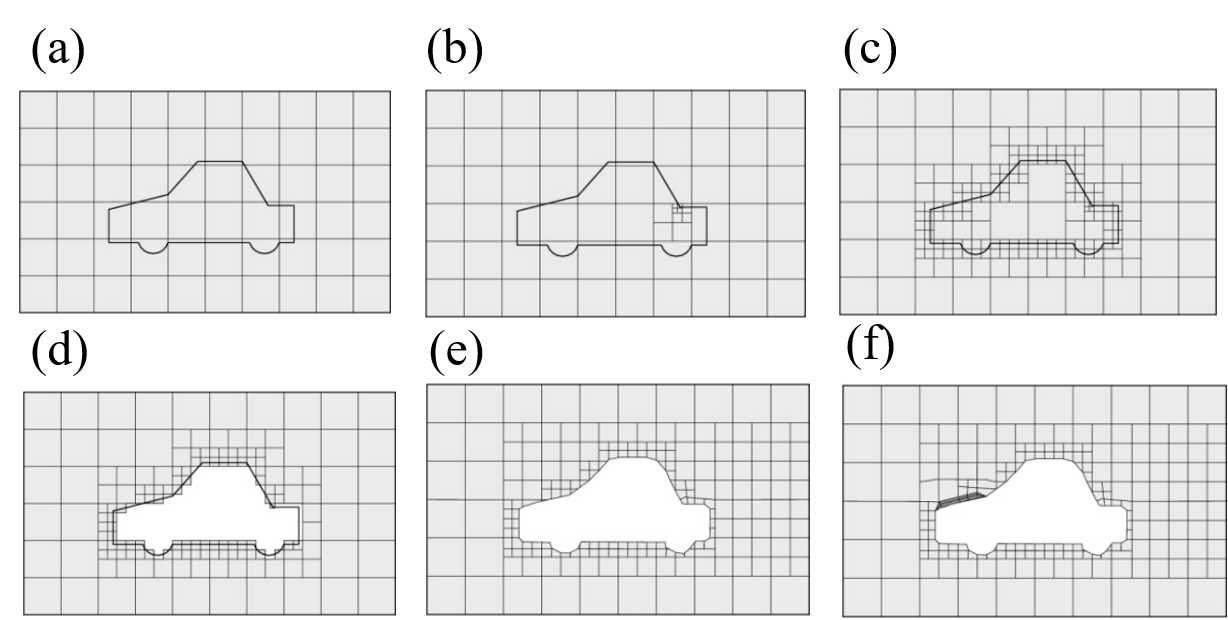
\includegraphics[width=12cm]{./pic/fig1.png}
\caption{メッシュ生成プロセス。(a)blockMeshによる基本メッシュの生成(b)特徴線付近の細分化(c)境界面の細分化(d)領域外の除去(e)界面適合(f)レイヤーメッシュの生成}
\end{center}
\end{figure}

\subsubsection{blockMeshDictのフォーマット}
{\bf blockMeshDict}とはblockMeshに関する諸設定を纏めたテキストファイルであり、{\bf ./system}に保存する。blockMeshはある程度複雑な形状のメッシュ生成が可能で、複雑な解析領域(図2中グレー領域)も解釈可能である。ただし、複雑形状及び空間はSTLファイルで用意することが一般的で、blockMeshに作ってもらいたい基本メッシュは、図2のような矩形であることが多い。本資料でも矩形領域及び立法格子を作成するための方法のみ紹介する。\par
\begin{lstlisting}[caption=blockMeshDictの基本フォーマット]
FoamFile
{
	version	2.0;
	format	ascii;
	class	dictionary;
	object	blockMeshDict;
}

minx		0;
maxx	1;
miny		0;
maxy	1;
minz		0;
maxz	1;

xm		(0 3 4 7);
xp		(1 2 6 5);
ym		(0 1 4 5);
yp		(2 3 6 7);
zm		(0 3 2 1);
zp		(4 5 6 7);

scale	1; 

vertices
(
	($minx $miny $minz)
	($maxx $miny $minz)
	($maxx $maxy $minz)
	($minx $maxy $minz)
	($minx $miny $maxz)
	($maxx $miny $maxz)
	($maxx $maxy $maxz)
	($minx $maxy $maxz)
	
);

blocks
(
	hex (0 1 2 3 4 5 6 7) (400 200 1) simpleGrading (1 1 1)
);


boundary
(
	inlet
	{
		type	patch;
		faces
		(
			$xm
		);
	}
	outlet
	{
		type	patch;
		faces
		(
			$xp
		);
	}
	wall
	{
		type	wall;
		faces
		(
			$ym
			$yp
		);
	}

	no_dim
	{
		type empty;
		faces
		(
			$zm
			$zp
		);
	}
);

mergePatchPairs
();
\end{lstlisting}\par
Listing2.1は基本的なblockMeshDictのフォーマットである。
\begin{itemize}
\item 7行目まではヘッダーと呼ばれるものであり、修正を加えることはない。
\item 9行目から21行目までのように、OpenFOAMは変数定義が可能である。
\item 24行目のscaleはメートルへの単位変換時に乗じる数値を定義している。例えば後に登場する数値をミリメートルで記載する場合は、ここで0.001を設定する。
\item verticesでは矩形領域の頂点座標を指定する。各点の定義の順番は重要で、ここを間違えると正しく矩形領域が定義できない。verticesで座標を直接入力するよりも、7-14行目のように各軸の定義域を指定して、良しなに座標定義の順番が定義されるようにした方が安全である。
\item blocksでは矩形領域と各軸の離散数、並びに計算格子の大きさを指定する。hex(0 1 2 3 4 5 6 7)は矩形領域を表しており、各数値はvertices中の頂点番号を意味している。従って(0 1 2 3 4 5 6 7)という定義とvertices中頂点の定義の順番は連携している訳であり、hex(0 1 2 3 4 5 6 7)のところは基本的に修正してはならない。(400 200 1)はx軸、y軸、z軸の離散数を表している。この場合、z軸方向の離散数が多く、z軸方向は離散化しない。このようにある軸を離散化せず、かつそれに直交する面で如何なる流束も生じないように設定すれば、OpenFOAMで2次元解析ができるようになる。simpleGrading (1 1 1)は各軸の計算格子幅の成長率を表す。図2.1のようにblockMeshの機能で不均質格子を生成することは稀なので、(1 1 1)の設定から変える必要はほぼ無い。
\item boundaryでは各面の名称と特性を定義する。Listing2.1中の「inlet」などは面の定義であり、$\{\}$内で諸設定を行う。typeでは壁面など面の特性を指定する。表2.1はtypeで指定できる特性の一覧である。facesでは対象の面を指定する。例えばinletのfacesに(0 3 4 7)を記入した場合、inletはx軸負側の面を指していることになる。63行目のwallのように、複数の面をfacesで指定することもできる。なお表2.1で説明している通り、typeでemptyを指定すればその面で流束は生じない。
\item mergePatchPairsでは、いわゆる界面境界を定義する。基本的な解析で使用することは少ないので、Listing2.1のように省略することが多い。
\end{itemize}

\begin{table}[t]
\begin{center}
\caption{境界のタイプ}
\begin{tabular}{ll} \hline
patch & パッチ。流入出境界条件で利用する。 \\
wall & 壁面境界。\\
symmetryPlane & 対称境界面。\\
cyclic & 周期境界条件。\\
cyclicAMI & 不整合周期境界条件。\\
wedge & 2次元軸対称。\\
empty & 2次元。 \\ \hline
\end{tabular}
\end{center}
\end{table}

blockMeshDictを編集後、解析ディレクトリで「blockMesh」と実行する。ただし、このときにcontrolDictファイルも保存していなければならない。controlDictについては3章で触れる。また、blockMeshの結果をfoamToVTKなどで出力する場合、fvSolutionとfvSchemesのファイルも必要になる。foamToVTKについては4章で、fvSolutionとfvSchemesについては3章で触れる。

\subsubsection{surfaceFeatureExtractDictのフォーマット}
{\bf surfaceFeatureExtractDict}とはsurfaceFeatureExtractに関する諸設定を纏めたテキストファイルであり、{\bf ./system}に保存する。前述の通り、surfaceFeatureExtractは特徴線を抽出する。このような処理は他の商用ソフトでも見られるが、OpenFOAMに限らず多くのソフトにおいて特徴線抽出のためのパラメータを調整することは稀である。従って特にこだわりがなければ下記のListing2.2をそのまま使うとよい。なお、9行目のgeo.stlは用意したCADファイルのことであり、9行目のみSTLファイル名に合わせて変更しなければならない。
\begin{lstlisting}[caption=surfaceFeatureExtractDictの基本フォーマット]
FoamFile
{
	version	2.0;
	format	ascii;
	class	dictionary;
	object	surfaceFeatureExtractDict;
}

geo.stl
{
	extractionMethod	extractFromSurface;
	extractFromSurfaceCoeffs
	{
		includedAngle	150;
	}

	writeObj	no;
}
\end{lstlisting}\par
この状態でsurfaceFeatureExtractを実行すると、{\bf ./constant/triSurface}にgeo.{\bf eMesh}というファイルが作成される。ちなみに特徴線がない非常に単純な形状であったとしても、surfaceFeatureExtractを実行しなければならない。この.eMeshファイルがないとsnappyHexMeshが実行できないためである。

\subsubsection{snappyHexMeshDictのフォーマット}
{\bf snappyHexMeshDict}とはsnappyHexMeshに関する諸設定を纏めたテキストファイルであり、{\bf ./system}に保存する。前述の通りsnappyHexMeshは図2.1(c)-(f)までの実行を担当するが、図2.1(c)-(e)のように途中で止めることも可能である。例えば直交格子のみで構成したいならば、図2.1(d)の完了時点で終了させればよい。
\begin{lstlisting}[caption=snappyHexMeshDictの基本フォーマット]
FoamFile
{
    version     2.0;
    format      ascii;
    class       dictionary;
    object      snappyHexMeshDict;
}

castellatedMesh true;
snap            true;
addLayers       true;

geometry
{
	geo.stl
	{
		type	triSurfaceMesh;
		name	geo;
	}
}

castellatedMeshControls
{
	maxLocalCells 100000;
	maxGlobalCells 2000000;
	minRefinementCells 0;
	maxLoadUnbalance 0.10;
	nCellsBetweenLevels 1;
	features
	(
		{
			file "geo.eMesh";
			level 0;
		}
	);

	refinementSurfaces
	{
		geo
		{
			level (0 0);
		}
		inlet
		{
			level (0 0);
		}
		outlet
		{
			level (0 0);
		}
		wall
		{
			level (0 0);
		}
		no_dim
		{
			level (0 0);
		}
	}

	resolveFeatureAngle	30;
	refinementRegions
	{}

	locationInMesh (2.003 0.003 0.0);
	allowFreeStandingZoneFaces true;

}

snapControls
{
	nSmoothPatch			3;
	tolerance				2.0;
	nSolveIter				30;
	nRelaxIter				5;
	nFeatureSnapIter		10;
	implicitFeatureSnape	false;
	explicitFeatureSnape	true;
	multiRegionFeatureSnape	false;
}
addLayersControls
{
    relativeSizes   true;
    expansionRatio  1.0;
    finalLayerThickness 0.3;
    minThickness    0.25;
    layers
    {
        "geo_side"
        {
            nSurfaceLayers  3;
        }
    }
    nGrow   0;
    featureAngle    130;
    maxFaceThicknessRatio   0.5;
    nSmoothSurfaceNormals   1;
    nSmoothThickness    10;
    minMedialAxisAngle  90;
    maxThicknessToMedialRatio    0.3;
    nSmoothNormals  3;
    slipFeatureAngle    30;
    nRelaxIter  5;
    nBufferCellsNoExtrude   0;
    nLayerIter  50;
    nRelaxedIter    20;
}
meshQualityControls
{
	maxNonOrtho			65;
	maxBoundarySkewness 20;
	maxInternalSkewness 4;
	maxConcave 			80;
	minVol 				1e-13;
	minTetQuality 		1e-15;
	minArea 			-1;
	minTwist 			0.02;
	minDeterminant 		0.001;
	minFaceWeight 		0.05;
	minVolRatio 		0.01;
	minTriangleTwist 	-1;
    errorReduction  0.75;
    nSmoothScale    4;
}
mergeTolerance 1e-6;
\end{lstlisting}\par
\begin{itemize}
\item snappyHexMeshで何をするかは9-11行目で指定する。castellatedMeshは図2.1(c)-(d)の処理、snapは図2.1(e)の処理、並びにaddlayersは図2.1(f)の処理のことを指す。
\item geometryでは読み込むCADファイルを定義する。Listing2.3のように、CADファイル名を記入し、trisurfaceMeshを指定する。nameはgeo.stlに変わる変数名であり、この後の処理で使うことができる。
\item castellatedMeshControlsでは、castellatedMeshの設定をする。
\begin{itemize}
\item maxLocalCellsは1コア当たりの許容できる最大計算格子数を意味する。
\item maxGlobalCellsは許容できる総計算格子数を意味する。
\item minRefinementCellsは図2.1(c)の再分割の繰り返しを制御する。繰り返し制御の途中、再分割が必要と判断されたメッシュの数がminRefinementCells以下になったとき、繰り返し計算は終了する。
\item maxLoadUnbalanceは並列計算時のコア毎の処理量のアンバランス性を設定するためにある。maxLoadUnbalanceが高いほど各コアの計算量を均等にしようとし、逆に低い場合は計算の配分を柔軟に割り当てることができる。
\item nCellsBetweenLevelsは少なくとも同じサイズのメッシュが並ぶ数を制御するためにある。この数が大きいほどメッシュサイズの急激な変化を緩和する。
\item featuresでは特徴線近傍のメッシュについて設定する。file部分で./constant/triSurfaceMeshにあるeMeshファイルを指定する(./constant/triSurface/*.eMeshのように相対パスで指定する必要はなく、ファイル名を記載するだけでよい)。また、レベルではメッシュのサイズを整数値で指定する(次項目参照)。
\item 前述の通り、snappyHexMeshはメッシュを8分木で管理する。メッシュを再分割するとき、元のメッシュの半分の長さ(体積は3次元空間の場合1/8)のメッシュを作成する。このとき、最も大きいメッシュ(木構造の根に相当)はblockMeshで生成された基本メッシュである。snappyHexMeshは、基本メッシュのサイズを「level 0」と呼び、そこから1段階ずつ小さくになるにつれlevelを1ずつ上げて呼ぶ。例えばfeaturesでlevel2と指定した場合、基本的にlevel 0のメッシュの1/64のサイズのメッシュが特徴線付近で生成される。なお、featuresがsnappyHexMeshDictで定義されていないとsnappyHexMesh実行時にエラーとなる。それゆえfeaturesの定義及びsurfaceFeatureExtractの実行は必須となる。
\item refinementSurfaceでは各面の分割レベルを設定できる。併せてSTLデータの面の定義も兼ねているので、たとえ基本メッシュからの再分割が不要であっても、refinementSurfaceには全ての面について記載しなければならない。定義の仕方はblockMesh及びSTLのsolidで設定した名前を指定し、それぞれに分割レベルを定義する。分割レベルはlevel $(x~y)$のように設定される。ここで$x<y$であり、面上のメッシュはlevel $x$から$y$のサイズとなるように自動調整される。再分割不要である場合はListing2.3のようにlevel (0 0)とすればよい。
\item 2つの境界面の成す角度が小さいとき、その間のメッシュは細かくしなければならない。角度の大小の閾値はresolveFeatureAngleで設定する。
\item refinementRegionsでは、領域に対するメッシュ細分化を指定できる。例えばカルマン渦における後流など、細かいメッシュが必要な領域が明らかな場合に指定する。
\item locationInMeshでは任意の解析領域内の座標を指定する。locationInMeshの設定によって、解析が内部流れか外部流れかが決まる。
\item allowFreeStandingZoneFacesについては現状よく分かっていない。ただし、trueにするのが一般的な模様。
\end{itemize}
\item snapControlsではsnap処理について設定する。なお、たとえsnapをfalseにしていたとしても、諸々のパラメータを入力しなければならない仕様になっている。snapをfalseにしているならば、これらパラメータが影響を及ぼすことはない。また、各パラメータの最適化は複雑なので、Listing2.3記載のデフォルト値を使うことが多い。
\begin{itemize}
\item nSmoothPatchは境界適合における平滑化反復回数である。
\item toleranceで境界適合の許容誤差を設定する。
\item nSolveIterでスナッピングの反復回数を指定する。
\item nRelaxIterでスナッピングのリラックス回数を指定する。
\item nFeatureSnapIterで特徴領域の反復回数を指定する。
\item implicitFeatureSnapeがtrueの場合は特徴領域のスナッピングを暗黙的に行い、explicitFeatureがtrueの場合は明示的に行う。
\item multiRegionFeatureSnapeで複数の領域のスナッピングを行うか指定する。
\end{itemize}
\item addLayersControlsでレイヤーに関する設定を行う。重要な設定だが、本例は立方格子を生成するためのサンプルも兼ねているので、ここでは紹介しない。ただし、addLayersがfalseでも「addLayersControls\{\}」は明記しなければならない。
\begin{itemize}
\item relativeSizesをtrueにした場合、レイヤー外メッシュサイズを相対値としてレイヤーメッシュサイズを指定できるようになる。
\item expansionRatioでレイヤーメッシュ成長率を指定する。
\item finalLayerThicknessは最外殻メッシュのサイズを指す。
\item minThicknessで下限サイズを指定する。
\item layersのディクショナリでレイヤーメッシュを作成する境界面を指定する。本例のように境界名とレイヤー数(nSurfaceLayers)を指定する。なお、境界はジオメトリの名前と境界面の名前で名づける。Listing2.3はジオメトリgeo(つまりgeo.stl)に含まれる境界名side(solid sideで定義されている面)の例であり、\"geo\_side\"のようにアンダーバーでつなげる。
\end{itemize}
\item meshQualityControlsでメッシュ品質の許容閾値を指定する。Listing2.3はデフォルト値であり、多くの場合このまま使う。
\item mergeToleranceの意味は現状分かっていない。ただし、1e-6よりも大きな数値を入れなければならないらしい。
\end{itemize}\par
snappyHexMeshDictを設定したら、snappyHexMeshを実行してメッシュを生成する。ただし、このときfvSolutionとfvSchemesのファイルも用意されていなければエラーとなる。

\subsubsection{その他処理と全体の流れ}
snappyHexMesh実行後、次にメッシュ品質のチェックを勧める。OpenFOAMはチェックのため処理を用意しており、{\bf checkMesh -constant}のコマンドを実行するだけでよい。なお、snappyHexMeshの結果は./constantに保存されており、checkMeshの後に続くオプション引数はそのことを意味している。\par
次に不要な境界を削除していく。snappyHexMeshを実行したとき、結果的に境界にメッシュが生成されないことがある(例えば内部流れにおけるblockMeshのいくつかの境界)。このような境界は不要なので、削除することが望ましい。OpenFOAMはそのためのコマンドとして、{\bf createPatch -overwrite}を用意している。なお、-overwriteはsnappyHexMeshの結果に上書きするためのもので、多くの場合指定される。また、createPatchの実行には下記の{\bf createPatchDict}が必要であり、実行時にはcreatePatchDictを{\bf ./system}フォルダに保存する。\par
最後に、連立一次方程式の係数行列のバンド幅を小さくするために、メッシュの定義の順序を並び変える。そのためには、{\bf renumberMesh -overwrite}を実行すればよい。
\begin{lstlisting}[caption=createPatchDictの基本フォーマット]
FoamFile
{
	version	2.0;
	format	ascii;
	class		dictionary;
	object		createPatchDict;
}

pointSync	false;
patches
(
);
\end{lstlisting}\par
最後にblockMeshからrenumberMeshまでの一連のコマンドを記す。
\begin{lstlisting}[caption=メッシュ作成手順]
blockMesh
surfaceFeatureExtract
snappyHexMesh -overwrite
checkMesh -constant
createPatch -overwrite
renumberMesh -overwrite
\end{lstlisting}\par

\section{解析条件の設定}

\end{document}
解析条件の設定はcontrolDictやfvSchemesなどのファイルで設定するが、ファイルに記述すべき内容は解法(simple法など)によって大きく異なり、しかもややこしい。例えば解法のsimpleFOAMは定常乱流解析をデフォルトとして考えているため、たとえ層流解析であっても乱流応力の収束などについてわざわざ指定しなければならない。そのため、解析をするときは一から解析条件設定のためのファイルを用意するのではなく、解法毎に用意されたファイルを引用することが多い。\par
とはいえ各ファイルの意味を理解することは重要なので、本章の初めに各ファイルの紹介をする。解法毎に用意された設定ファイルはその後に回す。

\subsection{解析条件設定ファイルの紹介}
\subsubsection{controlDict}
{\bf controlDict}とは解析の時間刻み幅や出力トリガー等を設定するファイルであり、{\bf ./system}に保存する。controlDictの各設定値の解釈は定常計算と非定常計算で異なる。\par
まず初めに定常計算におけるcontrolDictのフォーマットを以下に示す。
\begin{lstlisting}[caption=定常計算におけるcontrolDictの基本フォーマット]
FoamFile
{
	version	2.0;
	format	ascii;
	class	dictionary;
	object	controlDict;
}
application	simpleFoam;
startFrom	startTime;
startTime	0;
stopAt	endTime;
endTime	1000;
deltaT	1;
writeControl	timeStep;
writeInterval	100;
purgeWrite	0;
writeFormat	ascii;
writePrecision	6;
writeCompression	off;
timeFormat	general;
timePrecision	6;
runTimeModifiable	true;
\end{lstlisting}
\begin{itemize}
\item applicationでは、利用するソルバー名(後述)を指定する。
\item controlDictでは、連立一次方程式の反復計算回数のことを時刻と呼んでいる。
\item startFromでは下記の何れかを選択し、開始時刻を指定する。
\begin{itemize}
\item latestTime:既に存在するデータの中で、最も遅い時刻(つまり最新時刻)から開始。これを選択すれば中断していた解析を再開することができる。
\item firstTime:既に存在する時刻データの中で、最も早い時刻から開始。
\item "startTime"で設定した時刻から開始。これを選択した場合は12行目のように数値を入力しなければならない。
\end{itemize}
\item stopAtでは下記の何れかを選択し、解析終了時刻を指定する。
\begin{itemize}
\item writeNow:現時刻の計算を終えてから、計算結果を書き出して停止。
\item noWriteNow:現時刻の計算を終えてから、計算結果を書き出さずに停止。
\item nextTime:次の計算結果の書き出し時刻(後述)で停止。
\item endTime:"endTime"で設定した時刻で終了。これを選択した場合は20行目のように数値を入力しなければならない。
\end{itemize}
\item 定常解析の場合、deltaT、つまり時間刻み幅は必ず1とする。
\item writeControl及びwriteIntervalで計算結果出力のタイミングを設定する。一般的にはwriteControlでtimeStepを選択し、writeIntervalでその間隔を設定する。
\item 出力結果の総メモリ制御のために、purgeWriteで出力の最大保存数を指定する。例えば数値Nと指定した場合、時系列出力結果のうち最新のN個のみ保存する。ただし、purgeWriteをゼロとした場合は全出力結果を保存する。
\item 計算結果ファイルフォーマットはwriteFormatで指定する(基本的にasciiでよい)。
\item writeFormatがasciiの場合、計算結果の数値の桁数はwritePrecisionで指定できる。
\item writeCompressionで、出力結果を都度圧縮するか否かを指定できる。指定にはon/offを使う。
\item 時刻の書式(例えば12.34なのか1.234e+1なのか)はtimeFormatで指定できる。generalとしておけばOpenFOAMがよしなに書式を選択してくれる。
\item 時刻数値の桁数はtimePrecisionで指定する。
\item 解析再開時にcontrolDictファイルを再読み込みして欲しい場合は、runTimeModifiableをtrueとする。基本的にtrueでよい。
\end{itemize}\par
非定常解析の場合、時間を秒で指定する。ただしwriteIntervalのみはタイムステップ数である。
\begin{lstlisting}[caption=非定常計算におけるcontrolDictの基本フォーマット]
FoamFile
{
    version     2.0;
    format      ascii;
    class       dictionary;
    object      controlDict;
}
application     icoFoam;
startFrom       latestTime;
startTime       0;
stopAt          endTime;
endTime         10;
deltaT          0.05;
writeControl    timeStep;
writeInterval   20;
purgeWrite      0;
writeFormat     ascii;
writePrecision  6;
writeCompression off;
timeFormat      general;
timePrecision   6;
runTimeModifiable true;
\end{lstlisting}

\subsubsection{transportProperties}
物性値の設定は{\bf transportProperties}ファイルで行う。このファイルは{\bf ./constant}に保存する。解析に必要な物性値は解析条件毎に異なる。例えば層流解析の場合は以下のように動粘性係数のみ指定すればよい。
\begin{lstlisting}[caption=transportPropertiesの例]
FoamFile
{
    version 2.0;
    format  ascii;
    class   dictionary;
    object  transportProperties;
}

nu  0.01;
\end{lstlisting}

\subsubsection{fvSchemes}
有限体積法において必要な離散化の設定は{\bf fvSchemes}ファイルで行う。このファイルは{\bf ./system}に保存する。\par
fvSchemesでは以下の離散化を設定する(フォーマット例は別の節で紹介する)。
\begin{itemize}
\item ddtSchemes:時間微分に関する離散化。以下のいずれかを設定。
\begin{itemize}
\item steadyState:定常解析の場合。
\item Euler:Euler法(1次精度)の場合。
\item CrankNicolson:クランク-ニコルソン法の場合。例えば「default CrankNikolson x」のように記載する。ここでxは[0,1]のパラメータであり、0ならばEuler法と同じ処理になる。
\item backward:後退差分(2次精度)の場合。
\end{itemize}
\item gradSchemes:セル界面上の勾配を計算するための補間方法。基本的にGauss linearにする。
\item divSchemes:発散項に関する離散化。
\item laplacianSchemes:ラプラシアンに関する離散化。基本的にGauss linear correctedとする。
\item interpolationSchemes:セル界面上の物理量を計算するための補間方法。基本的にlinearとする。
\item snGradSchemes:非直交補正に関する設定。基本的にcorrectedとする。
\end{itemize}
離散化方法は物理量毎に指定できる。また、デフォルトの指定も可能であり、明示的に指定されなかった物理量はデフォルトの方法で離散化される。\par
上記離散化の中で最も重要なものはdivSchemesである。物理量Xに関する発散項はdiv(X)と書かれる。一方でdiv(phi, X)はXによるphiの移流を意味する。流体解析において対流項の取り扱いは重要であるため、div(phi, X)の設定には特に注意しなければならない。以下にdivSchemesで設定できる方法を示す。
\begin{itemize}
\item linear:線形補間(中心差分、2次精度)。
\item upwind:1次風上差分。
\item linearUpwind:線形風上差分(2次精度)。
\item QUICK:QUICKスキーム(2次精度)。
\item Minmod:minmod制限関数(2次精度TVD)。
\item SuperBee:superbee制限関数(2次精度TVD)。
\item vanLeer:van Leer制限関数(2次精度TVD)。
\item vanAlbada:van Albada制限関数(2次精度TVD)。
\item UMIST:UMIST制限関数(2次精度TVD)。
\item MUSCL:Monotonized central difference制限関数(2次精度TVD)。
\item limitedLinear:線形補間にTVD制限をつけたもの。安定性を調整するための[0, 1]のパラメータを設定する必要がある。例えば「default limitedLinear 1」のように指定する。このパラメータが大きいほど安定性は高い。ベクトル用の離散化ではlimitedLinearVを用いる。
\end{itemize}
なお、計算を安定化するためにboundedという指定ができ、例えば「bounded Gauss upwind」のように設定する。定常解析時にこれを利用することが推奨されている。bounded以外にもGaussというものを指定することが多いが、私はまだこの意味を理解していない。

\subsubsection{fvSolution}
{\bf fvSolution}では線形代数ソルバーの解法を設定する。解法は物理量毎に設定することができる。いくつか解法は用意されているが、圧力に対してはPCG(前処理付きCG法)、それ以外はPBiCG(前処理付きBiCG法)を使えばよい。以下はsimple法における例である。
\begin{lstlisting}[caption=fvSolutionの例]
FoamFile
{
    version     2.0;
    format      ascii;
    class       dictionary;
    object      fvSolution;
}
solvers
{
    p
    {
        solver          PCG;
        preconditioner  DIC;
        tolerance       1e-06;
        relTol          0.01;
    }
    U
    {
        solver          PBiCG;
        smoother        DILU;
        tolerance       1e-05;
        relTol          0.1;
    }
}
SIMPLE
{
    nNonOrthogonalCorrectors 2;
    pRefPoint   (40 0 0);
    pRefValue   0;
    residualControl
    {
        p   1e-3;
        U   1e-3;
    }
}
relaxationFactors
{
    fields
    {
        p   0.3;
    }
    equations
    {
        U   0.7;
    }
}
\end{lstlisting}
\begin{itemize}
\item solversで連立一次方程式の解法を設定する。基本的に前処理は上記のものを使うとよい。toleranceは残差の閾値、refTolは残差比(初期残差に対する比率)であり、これらよりも低くなれば収束したと判定する。
\item 本例ではSIMPLE法を用いている。
\begin{itemize}
\item nNonOrthogonalCorrectorsは格子の非直交性に関わる数値であり、基本的に2とする。
\item pRefPointは基準圧力とする位置、pRefValueは基準圧力値である。圧力境界条件がある場合は参照されない。
\item residualControlは収束判定値である。
\end{itemize}
\item relaxationFactorsは連立一次方程式ソルバーの緩和係数である。fieldsとequationsの違いは分からない。
\end{itemize}

\subsubsection{初期条件と境界条件の設定}
B.C.(境界条件)とI.C.(初期条件)の設定は{\bf ./0}で行う。

\end{document}


















\section{ポスト処理}



\section*{付録}
\subsection*{OpenFOAMの環境変数一覧}
\begin{itemize}
\item FOAM\_TUTRIALS:チュートリアルケースのあるパス名。tutとコマンドを打てばこの場所に移動できる。
\end{itemize}
\subsection*{OpenFOAMの特殊コマンド一覧}
\begin{itemize}
\item tut:「cd \$FOAM\_TUTRIALS」と等しい。
\end{itemize}












